\documentclass[11pt,a4paper]{article}
\usepackage[utf8]{inputenc}
\usepackage[francais]{babel}

\usepackage{amsmath}
\usepackage{amsfonts}
\usepackage{amssymb}
\usepackage{graphicx}
\usepackage[left=2cm,right=2cm,top=2cm,bottom=2cm]{geometry}

\title{Écoulements biologiques}
\author{Tiago Lobato Gimenes \\ Chongmo Liu}

\numberwithin{equation}{subsection}
\numberwithin{figure}{subsection}

\begin{document}

\maketitle

%
%		INTRODUCTION
%
\section*{Introduction}

TODO: ecrire introduction

%
%		SECTION
%
\section{Problème proposé}

Le problème proposé a été d'étudier les écoulements biologiques, plus précisément, l'écoulement sanguin dans des petites artères.
 
Le modèle mathématique proposé pour résoudre ce problème a eu une évolution au cours du modal. Premièrement nous avons commencé avec un modèle simple d'écoulement d'un fluide incompressible dans un tube avec des parois fixes. Nous avons aussi supposé que le nombre de Reynolds de  l'écoulement est petit et que les forces volumiques sont négligeables, ce que nous a permit d'utiliser le modèle suivante:
\begin{equation}
\begin{aligned}
& -\nu \Delta u + \nabla p = 0 \\
& -\mathrm{div}\;u = 0 \label{Stokes}
\end{aligned}
\end{equation}

\section{Le cas du rectangle 2D}
Nous avons décidé, d'abord, de commencer par simulant le problème \ref{Stokes} dans le rectangle $\Omega = \{(x,y) \in \mathbb{R}^2 \;t.q\; 0 \leq x \leq L, \; -R/2 \leq y \leq R/2\}$, c'est-à-dire, en deux dimensions. Les conditions au limites du problème que nous avons utilisé ont été:
\begin{equation}
\begin{aligned}
& \underline{u}(x,-R) = \underline{0} \\
& \underline{u}(x, R) = \underline{0} \\
& \underline{u}(0,y) = \left(R^2 - y^2, 0\right) \\
& \nu\frac{\partial\underline{u}}{\partial n}(L,y) = p.\underline{n}
\end{aligned} \label{LimitesClassiques}
\end{equation}

La formulation variationnelle du problème \ref{Stokes} avec les conditions \ref{LimitesClassiques} devient, donc, la suivante:
\begin{equation}
\nu \int\limits_\Omega \nabla \underline{u} \nabla \underline{v} \;\mathrm{d}\Omega - \int\limits_\Omega p\nabla v \; \mathrm{d}\Omega = 0 \label{FormuleVariationnelleSansTranspose}
\end{equation}

où $v$ est une fonction nulle sur touts les bords du rectangle $\Omega$ sauf sur la bord où $x = L$.

\subsection{Simulation de la formulation variationnelle \ref{FormuleVariationnelleSansTranspose}}

En faisant la simulation de la formulation variationnelle \ref{FormuleVariationnelleSansTranspose} avec les conditions aux limites \ref{LimitesClassiques} nous avons comme résultat les figures \ref{StokesConditionsClassiques} et \ref{StokesCondtiionsClassiquesPression}, ce que correspond bien à l'écoulement de Poiseuille, solution analytique dans ce cas.

\begin{figure}[H]
\centering
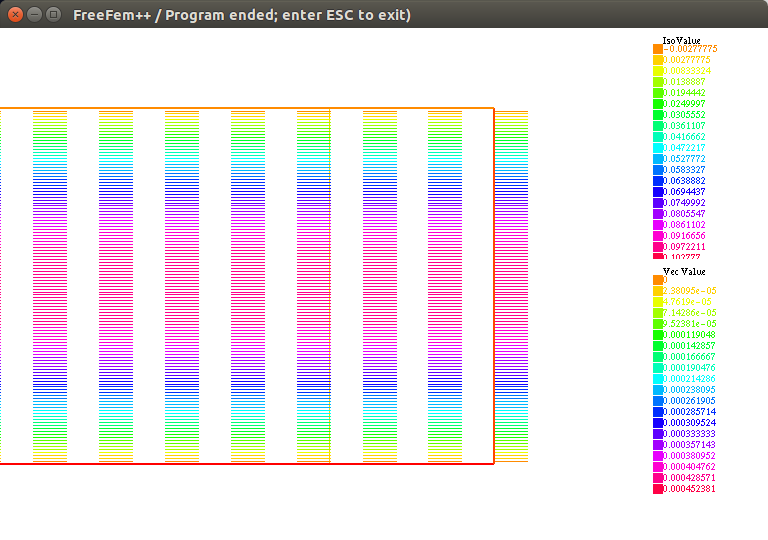
\includegraphics[scale=0.4]{StokesConditionsClassiques.png}
\caption{Profil de la vitesse pour le problème variationnelle \ref{FormuleVariationnelleSansTranspose} avec les conditions \ref{LimitesClassiques}}
\label{StokesConditionsClassiques}
\end{figure}

\begin{figure}[H]
\centering
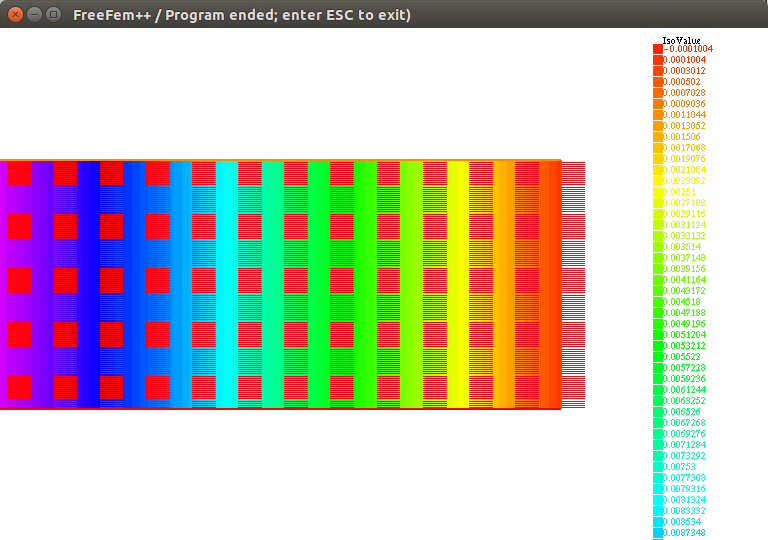
\includegraphics[scale=0.4]{StokesConditionsClassiquesPression.png}
\caption{Profil du gradient de pression pour le problème variationnelle \ref{FormuleVariationnelleSansTranspose} avec les conditions \ref{LimitesClassiques}}
\label{StokesCondtiionsClassiquesPression}
\end{figure}

Nous avons aussi fait une maillage non régulière qui est plus dense dans les endroit où la pression varie le plus. Les résultats peuvent êtres vus dans les figures \ref{StokesConditionsClassiquesVitessesIrregulier} et \ref{StokesConditionsClassiquesPressionIrregulier}.

\begin{figure}
\centering
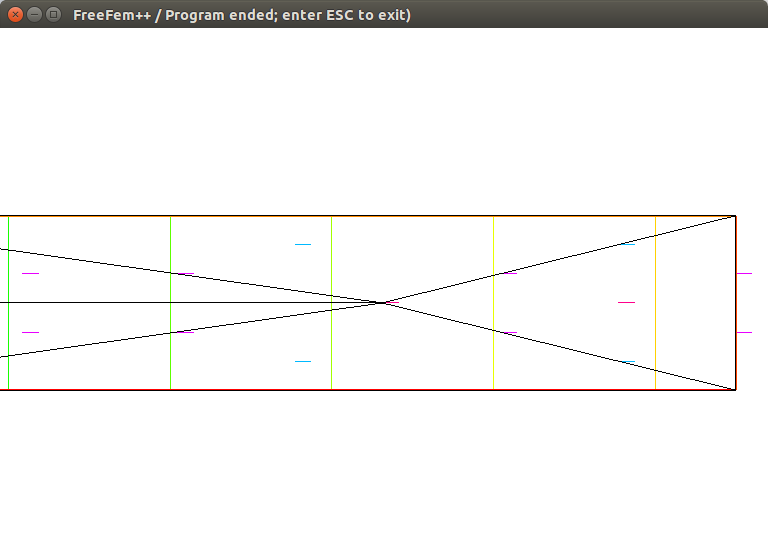
\includegraphics[scale=0.4]{StokesConditionsClassiquesVitessesIrregulier.png}
\caption{Profil des vitesses pour le problème variationnelle \ref{FormuleVariationnelleSansTranspose} avec les conditions \ref{LimitesClassiques} dans une maillage irrégulière}
\label{StokesConditionsClassiquesVitessesIrregulier}
\end{figure}	

\begin{figure}
\centering
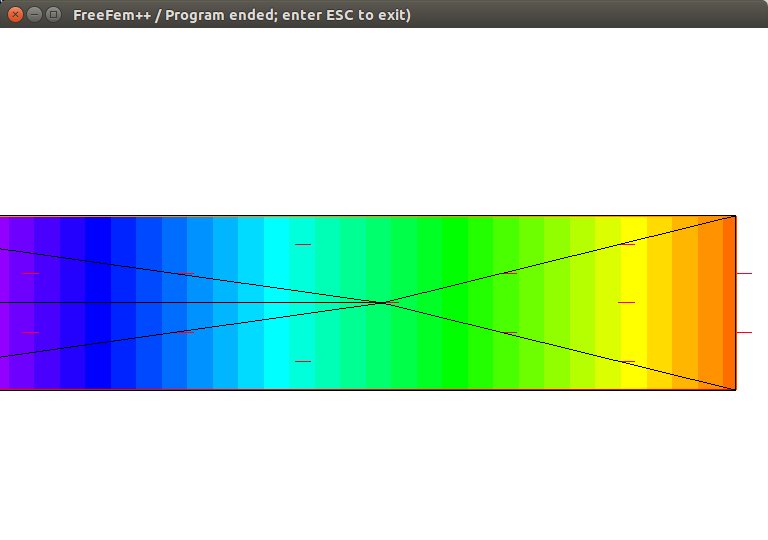
\includegraphics[scale=0.4]{StokesConditionsClassiquesPressionIrregulier.png}
\caption{Profil du gradient de pression pour le problème variationnelle \ref{FormuleVariationnelleSansTranspose} avec les conditions \ref{LimitesClassiques} dans une maillage irrégulière}
\label{StokesConditionsClassiquesPressionIrregulier}
\end{figure}

\subsection{Simulation de la formulation variationnelle \ref{FormuleVariationnelleAvecTranspose}}

La formulation variationnelle \ref{FormuleVariationnelleSansTranspose} peut avoir une autre forme parce que $\mathrm{div} u = 0$ et donc la formulation variationnelle suivante admet la même solution que la formulation \ref{FormuleVariationnelleSansTranspose}.
\begin{equation}
\begin{aligned}
\nu \int\limits_\Omega \left(\nabla \underline{u} + \nabla \underline{u}^t\right) \nabla \underline{v} \;\mathrm{d}\Omega - \int\limits_\Omega p\nabla v \; \mathrm{d}\Omega = 0
\label{FormuleVariationnelleAvecTranspose}
\end{aligned}
\end{equation}

Prenons $v$, la même fonction que nous avons utilisé ci-dessus. En intégrant par parties et en développant le calcul, nous arrivons aux conditions aux bords.
\begin{equation}
\begin{aligned}
& \underline{u}(x,-R) = \underline{0} \\
& \underline{u}(x, R) = \underline{0} \\
& \underline{u}(0,y) = \left(R^2 - y^2, 0\right) \\
& \nu\left(\frac{\partial\underline{u}}{\partial n}(L,y) + \frac{\partial\underline{u}}{\partial n}^t(L,y)\right) = p.\underline{n}
\end{aligned} \label{Limites}
\end{equation}

En simulant la formule variationnelle \ref{FormuleVariationnelleAvecTranspose} avec les conditions aux bords \ref{Limites} nous avons les figures \ref{StokesLimitesTransposeVitesses} et \ref{StokesLimitesTransposePression}.

\begin{figure}[h]
\centering
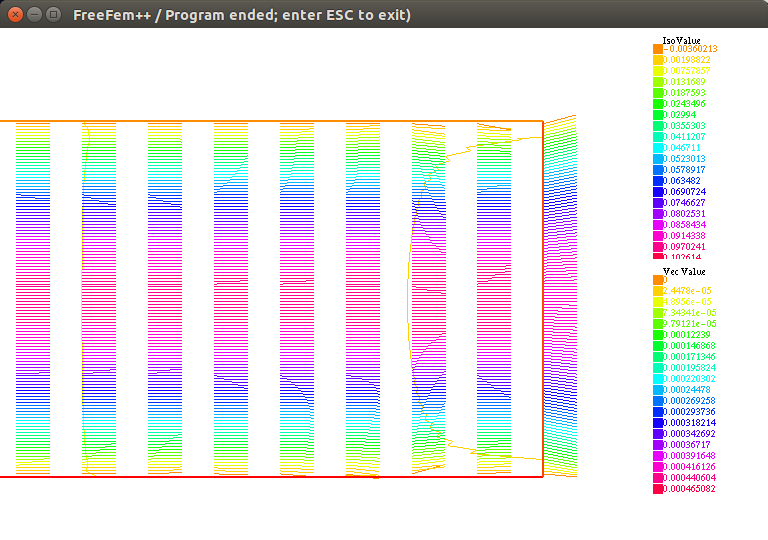
\includegraphics[scale=0.4]{StokesConditionsTransposeVitesses.png}
\caption{Profil des vitesses pour le problème variationnelle \ref{FormuleVariationnelleAvecTranspose} avec les conditions \ref{Limites}}
\label{StokesLimitesTransposeVitesses}
\end{figure}

\begin{figure}[h]
\centering
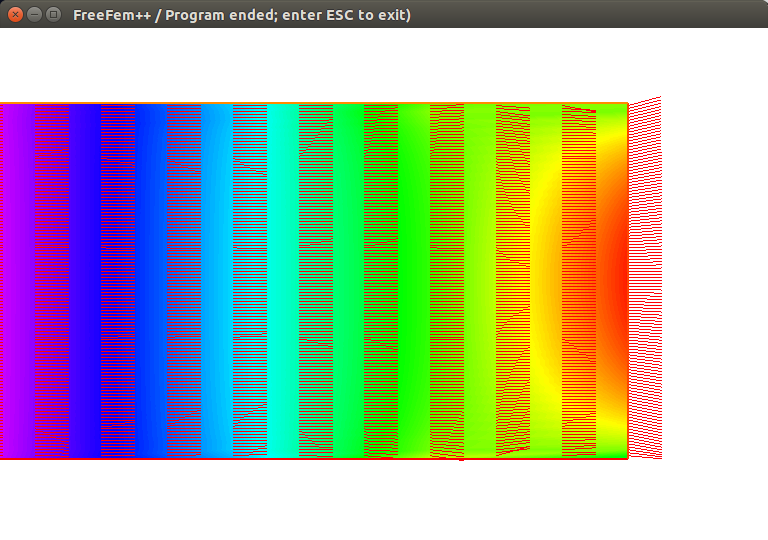
\includegraphics[scale=0.4]{StokesConditionsTransposePression.png}
\caption{Profil du gradient de pression pour le problème variationnelle \ref{FormuleVariationnelleAvecTranspose} avec les conditions \ref{Limites}}
\label{StokesLimitesTransposePression}
\end{figure}

Nous avons aussi fait une maillage non régulière qui est plus dense dans les endroit où la pression varie le plus. Les résultats peuvent êtres vus dans les figures \ref{StokesLimitesTransposeVitessesIrregulier} et \ref{StokesLimitesTransposePressionIrregulier}.

\begin{figure}[h]
\centering
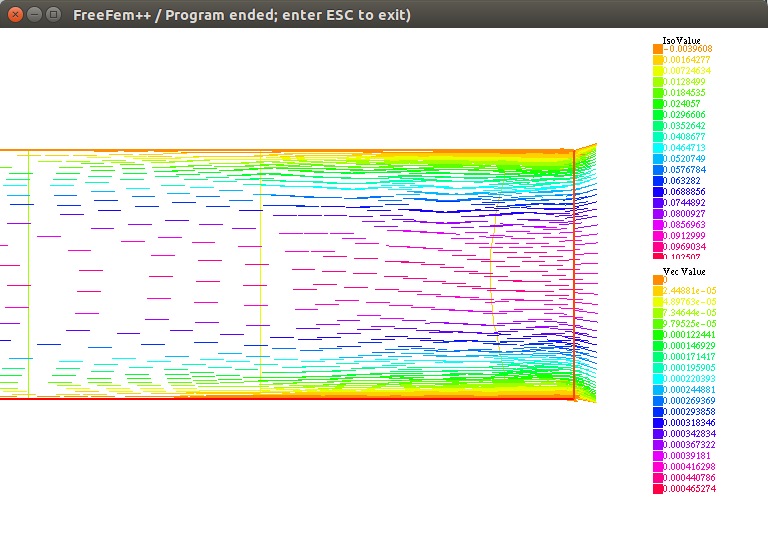
\includegraphics[scale=0.4]{StokesLimitesTransposeVitessesIrregulier.png}
\caption{Profil des vitesses pour le problème variationnelle \ref{FormuleVariationnelleAvecTranspose} avec les conditions \ref{Limites} dans une maillage irrégulière}
\label{StokesLimitesTransposeVitessesIrregulier}
\end{figure}

\begin{figure}[h]
\centering
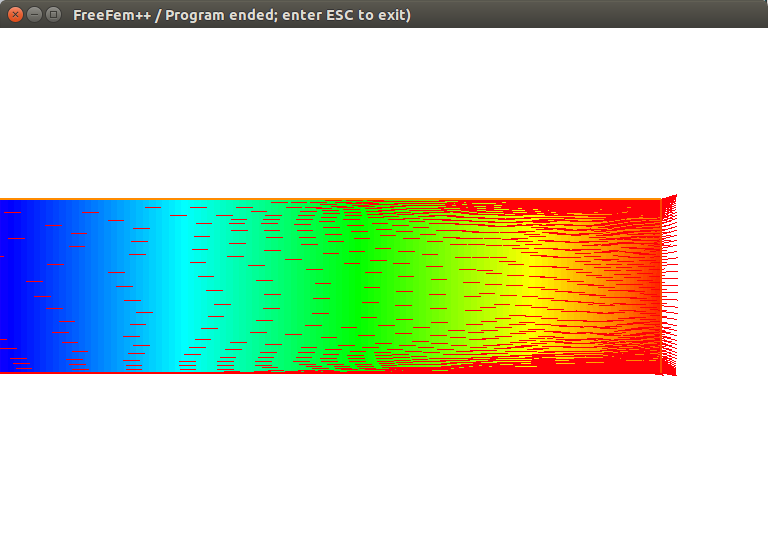
\includegraphics[scale=0.4]{StokesLimitesTransposePressionIrregulier.png}
\caption{Profil du gradient de pression pour le problème variationnelle \ref{FormuleVariationnelleAvecTranspose} avec les conditions \ref{Limites} dans une maillage irrégulière}
\label{StokesLimitesTransposePressionIrregulier}
\end{figure}

%
%		SECTION
%
\section{Le cas du cylindre 3D}

Pour résoudre le cas tridimensionnel nous avons supposé qu'il y a une symétrie axial, ce que nous rendre possible la décomposition du problème en 3D en 2D. Avec notre supposition de symétrie coaxiale, les formulations variationnelles \ref{FormuleVariationnelleAvecTranspose} et \ref{FormuleVariationnelleSansTranspose} deviennent, en coordonnées polaires, les formulations \ref{FormuleVariationnelleAvecTransposeCylindrique} et \ref{FormuleVariationnelleSansTransposeCylindrique} respectivement.
\begin{equation}
\begin{aligned}
& 2\pi\int\limits_0^r\int\limits_0^L \left(\frac{\partial u_r}{\partial r}\frac{\partial v_r}{\partial r} + \frac{\partial u_r}{\partial z}\frac{\partial v_r}{\partial z} + \frac{u_rv_r}{r^2} + \frac{\partial u_z}{\partial r}\frac{\partial v_z}{\partial r} + \frac{\partial u_z}{\partial z}\frac{\partial v_z}{\partial z}\right)r\mathrm{drdz}  \quad- \\
& 2\pi\int\limits_0^r\int\limits_0^L \left(p\left[\frac{\partial v_r}{\partial r} + \frac{v_r}{r} + \frac{\partial v_z}{\partial z}\right] - q\left[\frac{\partial u_r}{\partial r} + \frac{u_r}{r} + \frac{\partial u_z}{\partial z}\right]\right) r\mathrm{drdz} = 0
\end{aligned} \label{FormuleVariationnelleSansTransposeCylindrique}
\end{equation}

\begin{equation}
\begin{aligned}
& 2\pi\int\limits_0^r\int\limits_0^L \left(\frac{\partial u_r}{\partial r}\frac{\partial v_r}{\partial r} + \frac{\partial u_r}{\partial z}\frac{\partial v_r}{\partial z} + \frac{u_rv_r}{r^2} + \frac{\partial u_z}{\partial r}\frac{\partial v_z}{\partial r} + \frac{\partial u_z}{\partial z}\frac{\partial v_z}{\partial z}\right)r\mathrm{drdz}  \quad+ \\
& 2\pi\int\limits_0^r\int\limits_0^L \left(\frac{\partial u_r}{\partial r}\frac{\partial v_r}{\partial r} + \frac{\partial u_z}{\partial r}\frac{\partial v_r}{\partial z} + \frac{u_rv_r}{r^2} + \frac{\partial u_r}{\partial z}\frac{\partial v_z}{\partial r} + \frac{\partial u_z}{\partial z}\frac{\partial v_z}{\partial z}\right)r\mathrm{drdz}  \quad+ \\
& 2\pi\int\limits_0^r\int\limits_0^L \left(p\left[\frac{\partial v_r}{\partial r} + \frac{v_r}{r} + \frac{\partial v_z}{\partial z}\right] - q\left[\frac{\partial u_r}{\partial r} + \frac{u_r}{r} + \frac{\partial u_z}{\partial z}\right]\right) r\mathrm{drdz} = 0
\end{aligned} \label{FormuleVariationnelleAvecTransposeCylindrique}
\end{equation}

où $\underline{u} = u_r\underline{e}_r + u_z\underline{e}_z$ et $\underline{v} = v_r\underline{e}_r + v_z\underline{e}_z$. Pour simuler les formules variationnelles \ref{FormuleVariationnelleAvecTransposeCylindrique} et \ref{FormuleVariationnelleSansTransposeCylindrique} nous avons utilisée la symétrie coaxiale pour simuler juste la moitié du cylindre, ce que nous donne les conditions \ref{ConditionsMoitieTubeAvecTranspose} et \ref{ConditionsMoitieTubeSansTranspose} pour les formules variationnelles \ref{FormuleVariationnelleAvecTransposeCylindrique} et \ref{FormuleVariationnelleSansTransposeCylindrique} respectivement.
\begin{equation}
\begin{aligned}
& \underline{u}(x,-R) = \underline{0} \\
& \nu\frac{\partial\underline{u}}{\partial n}(x,0) = p.\underline{n} \\
& \underline{u}(0,y) = \left(R^2 - y^2, 0\right) \\
& \nu\frac{\partial\underline{u}}{\partial n}(L,y) = p.\underline{n}
\end{aligned} \label{ConditionsMoitieTubeSansTranspose}
\end{equation}

\begin{equation}
\begin{aligned}
& \underline{u}(x,-R) = \underline{0} \\
& \nu\left(\frac{\partial\underline{u}}{\partial n}(x,0) + \frac{\partial\underline{u}}{\partial n}^t(x,0)\right) = p.\underline{n} \\
& \underline{u}(0,y) = \left(R^2 - y^2, 0\right) \\
& \nu\left(\frac{\partial\underline{u}}{\partial n}(L,y) + \frac{\partial\underline{u}}{\partial n}^t(L,y)\right) = p.\underline{n}
\end{aligned} \label{ConditionsMoitieTubeAvecTranspose}
\end{equation}

\subsection{Simulation de la formule variationnelle \ref{FormuleVariationnelleSansTransposeCylindrique}}

En utilisant la formule variationnelle \ref{FormuleVariationnelleSansTransposeCylindrique} et les conditions aux bords \ref{ConditionsMoitieTubeSansTranspose} nous arrivons au figures \ref{StokesClassiqueVitessesCylindrique} et \ref{StokesClassiquePressionCylindrique}.

\begin{figure}
\centering
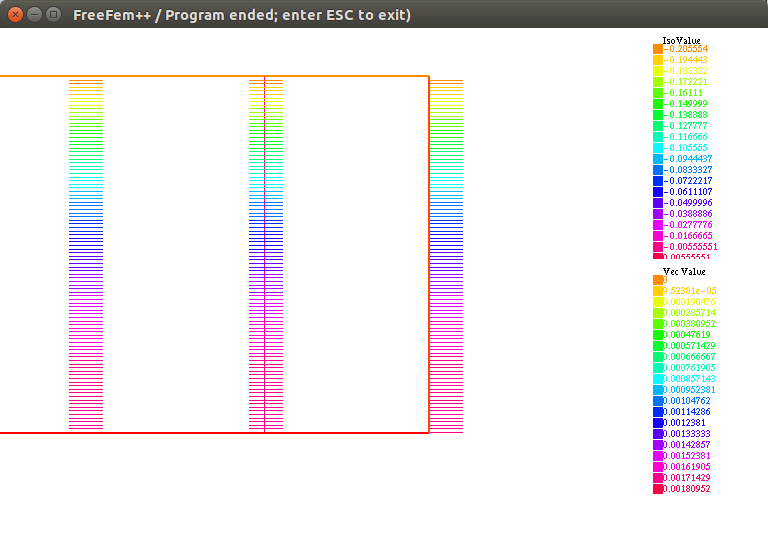
\includegraphics[scale=0.4]{StokesClassiqueVitessesCylindrique.png}
\caption{Profil des vitesses pour le problème variationnelle \ref{FormuleVariationnelleSansTransposeCylindrique} avec les conditions \ref{ConditionsMoitieTubeSansTranspose}}
\label{StokesClassiqueVitessesCylindrique}
\end{figure}

\begin{figure}
\centering
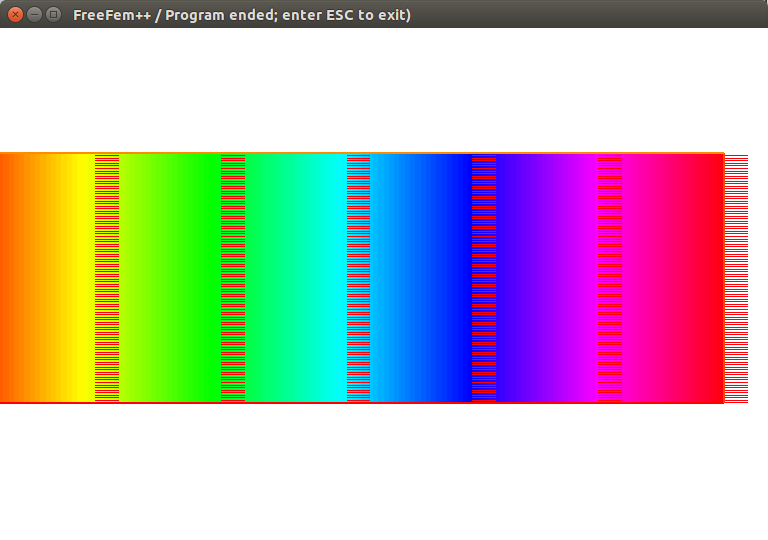
\includegraphics[scale=0.4]{StokesClassiquePressionCylindrique.png}
\caption{Profil du gradient de pression pour le problème variationnelle \ref{FormuleVariationnelleSansTransposeCylindrique} avec les conditions \ref{ConditionsMoitieTubeSansTranspose}}
\label{StokesClassiquePressionCylindrique}
\end{figure}

Nous avons aussi fait une maillage non régulière qui est plus dense dans les endroit où la pression varie le plus. Les résultats peuvent êtres vus dans les figures \ref{StokesClassiqueVitessesCylindriqueIrregulier} et \ref{StokesClassiquePressionCylindriqueIrregulier}

\begin{figure}
\centering
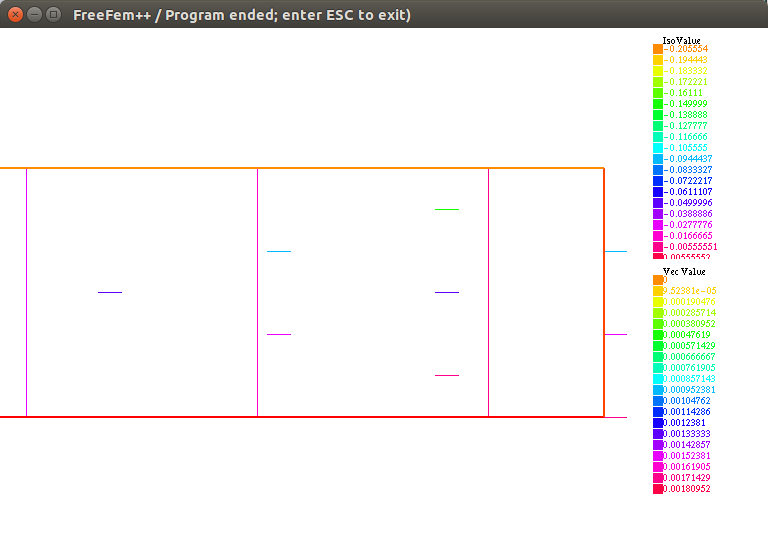
\includegraphics[scale=0.4]{StokesClassiqueVitessesCylindriqueIrregulier.png}
\caption{Profil des vitesses pour le problème variationnelle \ref{FormuleVariationnelleSansTransposeCylindrique} avec les conditions \ref{ConditionsMoitieTubeSansTranspose} dans une maillage irrégulière}
\label{StokesClassiqueVitessesCylindriqueIrregulier}
\end{figure}

\begin{figure}
\centering
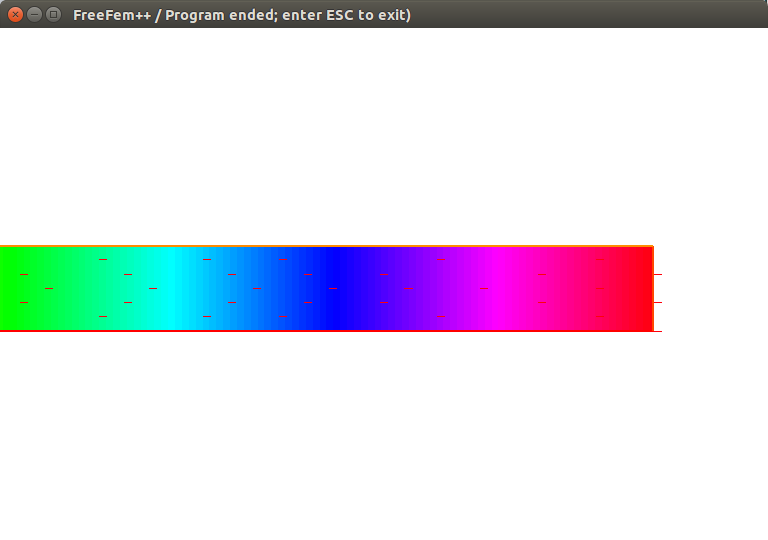
\includegraphics[scale=0.4]{StokesClassiquePressionCylindriqueIrregulier.png}
\caption{Profil du gradient de pression pour le problème variationnelle \ref{FormuleVariationnelleSansTransposeCylindrique} avec les conditions \ref{ConditionsMoitieTubeSansTranspose} dans une maillage irrégulière}
\label{StokesClassiquePressionCylindriqueIrregulier}
\end{figure}

\subsection{Simulation de la formule variationnelle \ref{FormuleVariationnelleAvecTransposeCylindrique}}

En utilisant la formule variationnelle \ref{FormuleVariationnelleAvecTransposeCylindrique} et les conditions aux bords \ref{ConditionsMoitieTubeAvecTranspose} nous arrivons au figures \ref{StokesLimitesVitesseCylindrique} et \ref{StokesLimitesPressionCylindrique}

\begin{figure}
\centering
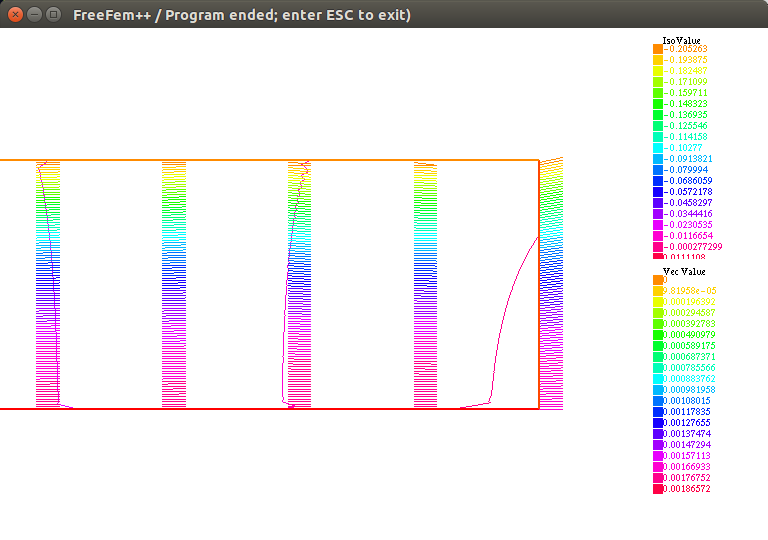
\includegraphics[scale=0.4]{StokesLimitesVitesseCylindrique.png}
\caption{Profil des vitesses pour le problème variationnelle \ref{FormuleVariationnelleAvecTransposeCylindrique} avec les conditions \ref{ConditionsMoitieTubeAvecTranspose}}
\label{StokesLimitesVitesseCylindrique}
\end{figure}

\begin{figure}	
\centering
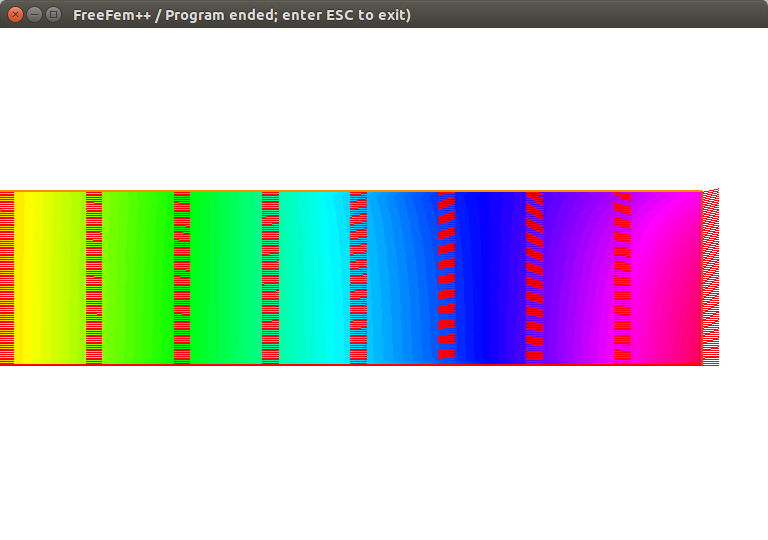
\includegraphics[scale=0.4]{StokesLimitesPressionCylindrique.png}
\caption{Profil du gradient des pressions pour le problème variationnelle \ref{FormuleVariationnelleAvecTransposeCylindrique} avec les conditions \ref{ConditionsMoitieTubeAvecTranspose}}
\label{StokesLimitesPressionCylindrique}
\end{figure}

Nous avons aussi fait une maillage non régulière qui est plus dense dans les endroit où la pression varie le plus. Les résultats peuvent êtres vus dans les figures \ref{StokesLimitesVitessesCylindriqueIrregulier} et \ref{StokesLimitesPressionCylindriqueIrregulier}

\begin{figure}
\centering
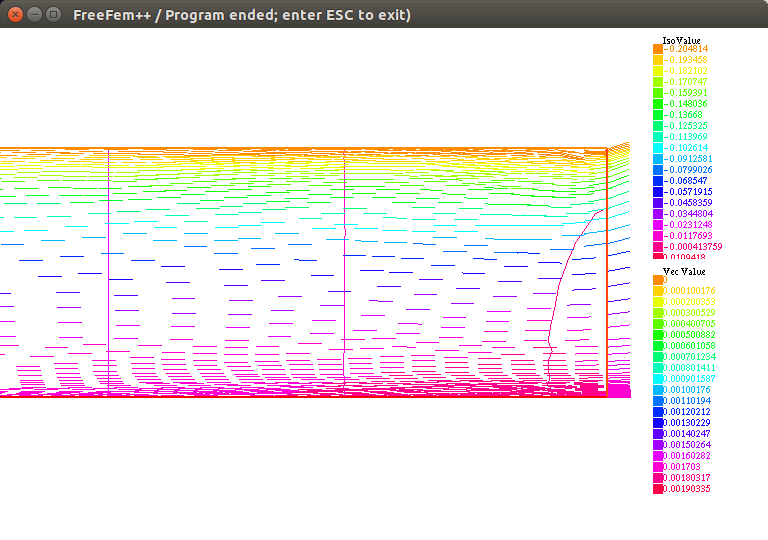
\includegraphics[scale=0.4]{StokesLimitesVitessesCylindriqueIrregulier.png}
\caption{Profil des vitesses pour le problème variationnelle \ref{FormuleVariationnelleAvecTransposeCylindrique} avec les conditions \ref{ConditionsMoitieTubeAvecTranspose} avec maillage irrégulière}
\label{StokesLimitesVitessesCylindriqueIrregulier}
\end{figure}

\begin{figure}
\centering
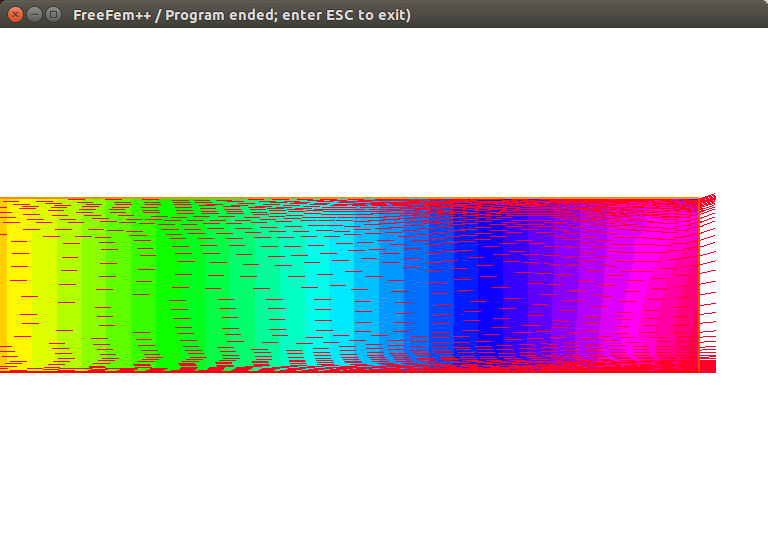
\includegraphics[scale=0.4]{StokesLimitesPressionCylindriqueIrregulier.png}
\caption{Profil du gradient des pressions pour le problème variationnelle \ref{FormuleVariationnelleAvecTransposeCylindrique} avec les conditions \ref{ConditionsMoitieTubeAvecTranspose} avec maillage irrégulière}
\label{StokesLimitesPressionCylindriqueIrregulier}
\end{figure}

%
%	SECTION
%
\section{Le cas 3D d'une forme symétrique non cylindrique}

Il a été proposé de faire l'étude d'un écoulement dans un objet qui avait toujours une symétrie coaxiale mais qui n'avait plus la forme d'un cylindre. 

\subsection{L'étude d'un cylindre avec une ellipse de révolution}

Une forme choisit pour faire cet étude a été un cylindre qui avait une ellipse de révolution. En utilisant la formule variationnelle \ref{FormuleVariationnelleSansTransposeCylindrique} et les conditions aux limites \ref{ConditionsMoitieTubeSansTranspose} nous avons les figures \ref{StokesClassiqueVitessesCylindreEllipse} et \ref{StokesClassiquePressionCylindreEllipse}

\begin{figure}[h]
\centering
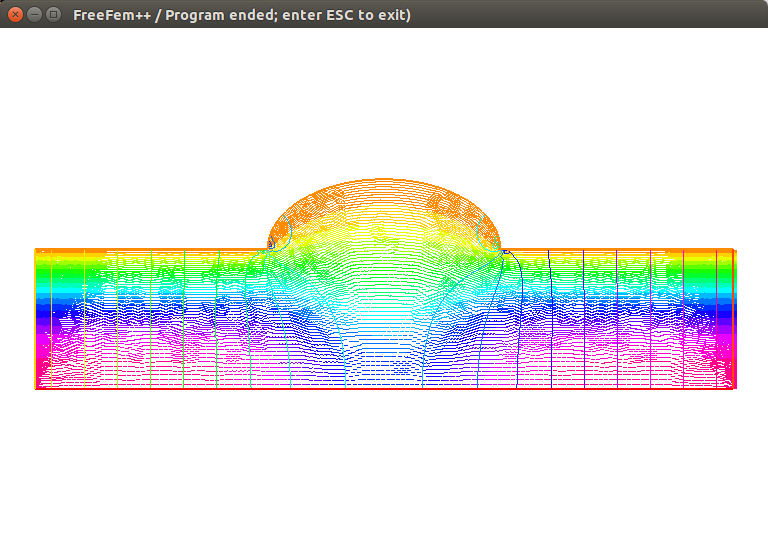
\includegraphics[scale=0.4]{StokesClassiqueVitessesCylindreEllipse.png}
\caption{Profil des vitesses pour le problème variationnelle \ref{FormuleVariationnelleSansTransposeCylindrique} avec les conditions \ref{ConditionsMoitieTubeSansTranspose} ajuste à la forme géométrique du cylindre + ellipse de révolution}
\label{StokesClassiqueVitessesCylindreEllipse}
\end{figure}

\begin{figure}[h]
\centering
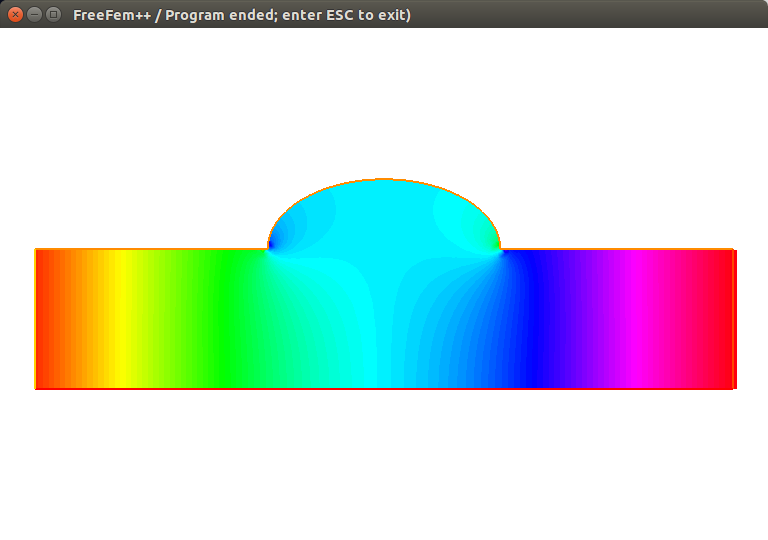
\includegraphics[scale=0.4]{StokesClassiquePressionCylindreEllipse.png}
\caption{Profil du gradient de pression pour le problème variationnelle \ref{FormuleVariationnelleSansTransposeCylindrique} avec les conditions \ref{ConditionsMoitieTubeSansTranspose} ajuste à la forme géométrique du cylindre + ellipse de révolution}
\label{StokesClassiquePressionCylindreEllipse}
\end{figure}

Nous avons aussi fait une maillage non régulière qui est plus dense dans les endroit où la pression varie le plus. Les résultats peuvent êtres vus dans les figures \ref{StokesClassiqueVitessesCylindreEllipseIrregulier} et \ref{StokesClassiquePressionCylindreEllipseIrregulier}

\clearpage

\begin{figure}[h]
\centering
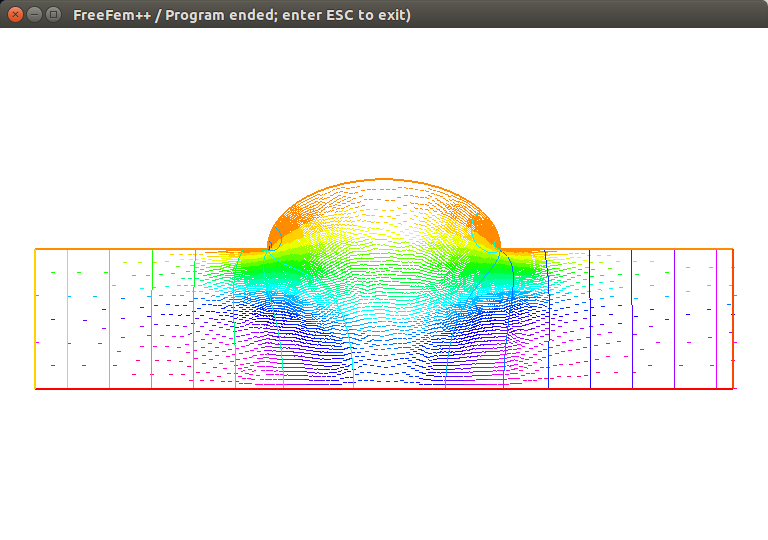
\includegraphics[scale=0.4]{StokesClassiqueVitessesCylindreEllipseIrregulier.png}
\caption{Profil des vitesses pour le problème variationnelle \ref{FormuleVariationnelleSansTransposeCylindrique} avec les conditions \ref{ConditionsMoitieTubeSansTranspose} ajuste à la forme géométrique du cylindre + ellipse de révolution pour un maillage irrégulier}
\label{StokesClassiqueVitessesCylindreEllipseIrregulier}
\end{figure}

\begin{figure}[h]
\centering
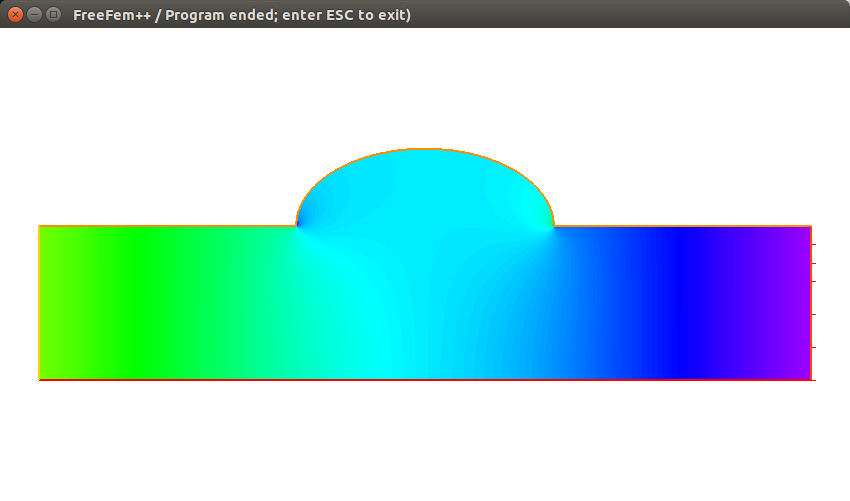
\includegraphics[scale=0.4]{StokesClassiquePressionCylindreEllipseIrregulier.png}
\caption{Profil du gradient de pression pour le problème variationnelle \ref{FormuleVariationnelleSansTransposeCylindrique} avec les conditions \ref{ConditionsMoitieTubeSansTranspose} ajuste à la forme géométrique du cylindre + ellipse de révolution pour un maillage irrégulier}
\label{StokesClassiquePressionCylindreEllipseIrregulier}
\end{figure}

\end{document}